%%%%%%%%%%%%%%%%%%%%%%%%%%%%%%%%%%%%%%%%%%%%%%%%%%%%%%%%%%%%%%%%%%%%%%%%%%%%%%%%
%2345678901234567890123456789012345678901234567890123456789012345678901234567890
%        1         2         3         4         5         6         7         8

\documentclass[letterpaper, 10 pt, conference]{ieeeconf}  % Comment this line out
                                                          % if you need a4paper
%\documentclass[a4paper, 10pt, conference]{ieeeconf}      % Use this line for a4
                                                          % paper

\IEEEoverridecommandlockouts                              % This command is only
                                                          % needed if you want to
                                                          % use the \thanks command
\overrideIEEEmargins
% See the \addtolength command later in the file to balance the column lengths
% on the last page of the document

\usepackage{url}
\usepackage{amsmath,amssymb}
\usepackage{float}
\usepackage{graphicx,subfigure}
\usepackage{color}
\usepackage[colorlinks=true,linkcolor=black]{hyperref}
\usepackage{breakurl}
\usepackage{cite}
\usepackage[ruled,linesnumbered]{algorithm2e}
\usepackage{ amssymb }
\usepackage{mathrsfs }
\setlength{\abovedisplayskip}{3pt}
\setlength{\belowdisplayskip}{3pt}

\newcommand{\minmax}{$\min\max$}
\newcommand{\pcomment}{\textcolor{blue}}% By Lifeng
\newcommand{\ie}{\emph{i.e.,}}
\newcommand{\tabincell}[2]{\begin{tabular}{@{}#1@{}}#2\end{tabular}}
\DeclareMathOperator{\Tr}{tr}

\newtheorem{theorem}{Theorem}
\newtheorem{lemma}{Lemma}
\newtheorem{definition}{Definition}
\newtheorem{proposition}{Proposition}
\newtheorem{problem}{Problem}

\title{\LARGE\bf Target Tracking with Signal Spoofing: Some Negative Results}%
\author{Zhongshun~Zhang, 
        Lifeng~Zhou
        and~Pratap~Tokekar% <-this % stops a space
\thanks{The authors are with the Department of Electrical \& Computer Engineering, Virginia Tech, USA. \texttt{\small \{zszhang, lfzhou, tokekar\}@vt.edu}.}%
\thanks{This material is based upon work supported by the National Science Foundation under Grant \#1566247.}}

\begin{document}

\maketitle
\thispagestyle{empty}
\pagestyle{empty}


%%%%%%%%%%%%%%%%%%%%%%%%%%%%%%%%%%%%%%%%%%%%%%%%%%%%%%%%%%%%%%%%%%%%%%%%%%%%%%%%
\begin{abstract}

The paper focuses on a pursuit-evasion game in probabilistic scenario, where both pursuer and evader positions are inexact and represented by the Gaussian distribution updated by a Kalman filter. The objective for the pursuer is to design the control command to capture the evader, i.e., keeps the inter target-robot distance bounded. Here, in order to escape from the pursuer, the  evader uses spoofing strategy to mislead the purser. 
% along with proofs of correctness and bounds on optimality.

\end{abstract}


%%%%%%%%%%%%%%%%%%%%%%%%%%%%%%%%%%%%%%%%%%%%%%%%%%%%%%%%%%%%%%%%%%%%%%%%%%
\section{Introduction}


%%%%%%%%%%%%%%%%%%%%%%%%%%%%%%%%%%%%%%%%%%%%%%%%%%%%%%%%%%%%%%%%%%%%%%%%%%
\section{Related Work} \label{sec:relwork}
Inspired by the predator-prey
behaviors in nature, pursuit-evasion games have been extensively studied in robotics\cite{pais2010pursuit}. In terms of differential games, pursuit-evasion problems have been formulated and studied in \cite{isaacs1999differential} and \cite{basar1999dynamic}. For a single pursuer and a single evader game\cite{sgall2001solution}, sufficient conditions are proposed for guaranteeing successful capture if both agents have the same equal maximum speeds and move within the non-negative quadrant of the plane with certain initial conditions. If both agents are restricted to moving with in a circular environment, upper and lower bounds of capture time have been calculated by assuming both agents can move optimally \cite{alonso1992lion}. As an extension and generalization work, a pursuit-evasion game involved with multiple pursers and a single evader has been proposed in\cite{kopparty2005framework} where the capture is guaranteed if the evader is initially located
inside a convex hull formulated by pursuers. 

A common theme of the works mentioned above is assuming a perfect geometry, i.e., the locations of both purser and evader are known. Here, we focus on the pursuit-evasion game problem where the exact positions of evader is unknown to the pursuer, i.e., only the maximum motion ability of evader or noisy position measurement can be acquired\cite{guibas1999visibility,rote2003pursuit,lavalle2006planning,jun2014pursuit,vander2014pursuit,aleem2015self}. The task for pursuer is to design a control strategy to eventually captures the evader. There are various ways of defining the "successful capture". Typically, in terms of uncertainty scenario, the objective for pursuer is to maintain a finite or pre-defined distance between the evader\cite{jun2014pursuit}. A game between two persons, a sheriff and thief has been presented in \cite{rote2003pursuit} where the sheriff only knows the approximate location of the thief, and the capture is due to the speed constraints of two players. Consider the uncertainty in bearing measurement, two classical pursuit-evasion games have been proposed in \cite{vander2014pursuit}. First, if two player are in the open plane, for any purser strategy, the evader can increase the distance with rate $\alpha$(linear in time) to the purser by an adversarial sensing model. Second, if the game is played inside a bounded circle area, the evader can escape from capture for any $\alpha>0$ when sensing uncertainty is considered. %A self-triggered pursuit strategy has been proposed in\cite{aleem2015self} where a tolerable upper-bounds on the sampling error is derived to guarantee the capture. 
Pursuit-evasion game with a probabilistic model has been proposed in \cite{jun2014pursuit} where both purser and evader positions are unknown and represented as a normal distribution evolving by a Kalman filter. And the boundedness of a distance of distributions between two players are guaranteed by resorting to sensor measurements only. 

\emph{KF tracking} estimation, distribution

\emph{Signal spoofing} A common theme in the mentioned works is how to design a pursuer's control strategy for successful capture. Here, we focus on a problem where evader formulates its escaping strategy to arbitrarily enlarge the distance between the purser and itself. Since only measurement of evader's position can be used by pursuer, the evader can adversarially add the spoofing signal on the measurement to mislead the purser. Thus, we propose an evader's spoofing strategy 

%%%%%%%%%%%%%%%%%%%%%%%%%%%%%%%%%%%%%%%%%%%%%%%%%%%%%%%%%%%%%%%%%%%%%%%%%%
\section{Problem Formulation} \label{sec:probform}

We assume that the position of the robot is known accurately using on-board sensors. The motion model of the target is given by:
\begin{equation}  \label{robot}
  x_{t+1}=Fx_{t}+Bu_t+\omega_t
\end{equation}   
where $x_{t}\in\mathbb{R}^2$ is the position of the target at step $t$, $u_t$ is the of control inputs at step $t$ and $w_t\sim \mathbb{N}(0, R_t)$ is the Gaussian process noise at time $t$. 

The robot was sensors to estimate the target's position. The measurement equation is:
\begin{equation}
  \label{measurement}
   z_t= Hx_t +v_t
\end{equation}
where  $v(t) \sim \mathcal{N}(0,Q_t)$.

The target can interference with the robot's sensor by adding spoofing signal to mislead the robot's estimate of the target's state. That is, $\tilde{z}_t$ is the actual measurement received by the robot, where $z_t$ would have been the measurement without spoofing. The spoofing signal $\epsilon$ increases the measurement error directly. 
\begin{equation}
  \label{spoofmeasurement}
 \tilde{z}_t= z_t + \epsilon_t
\end{equation}

\begin{figure}[H]
  \centering
  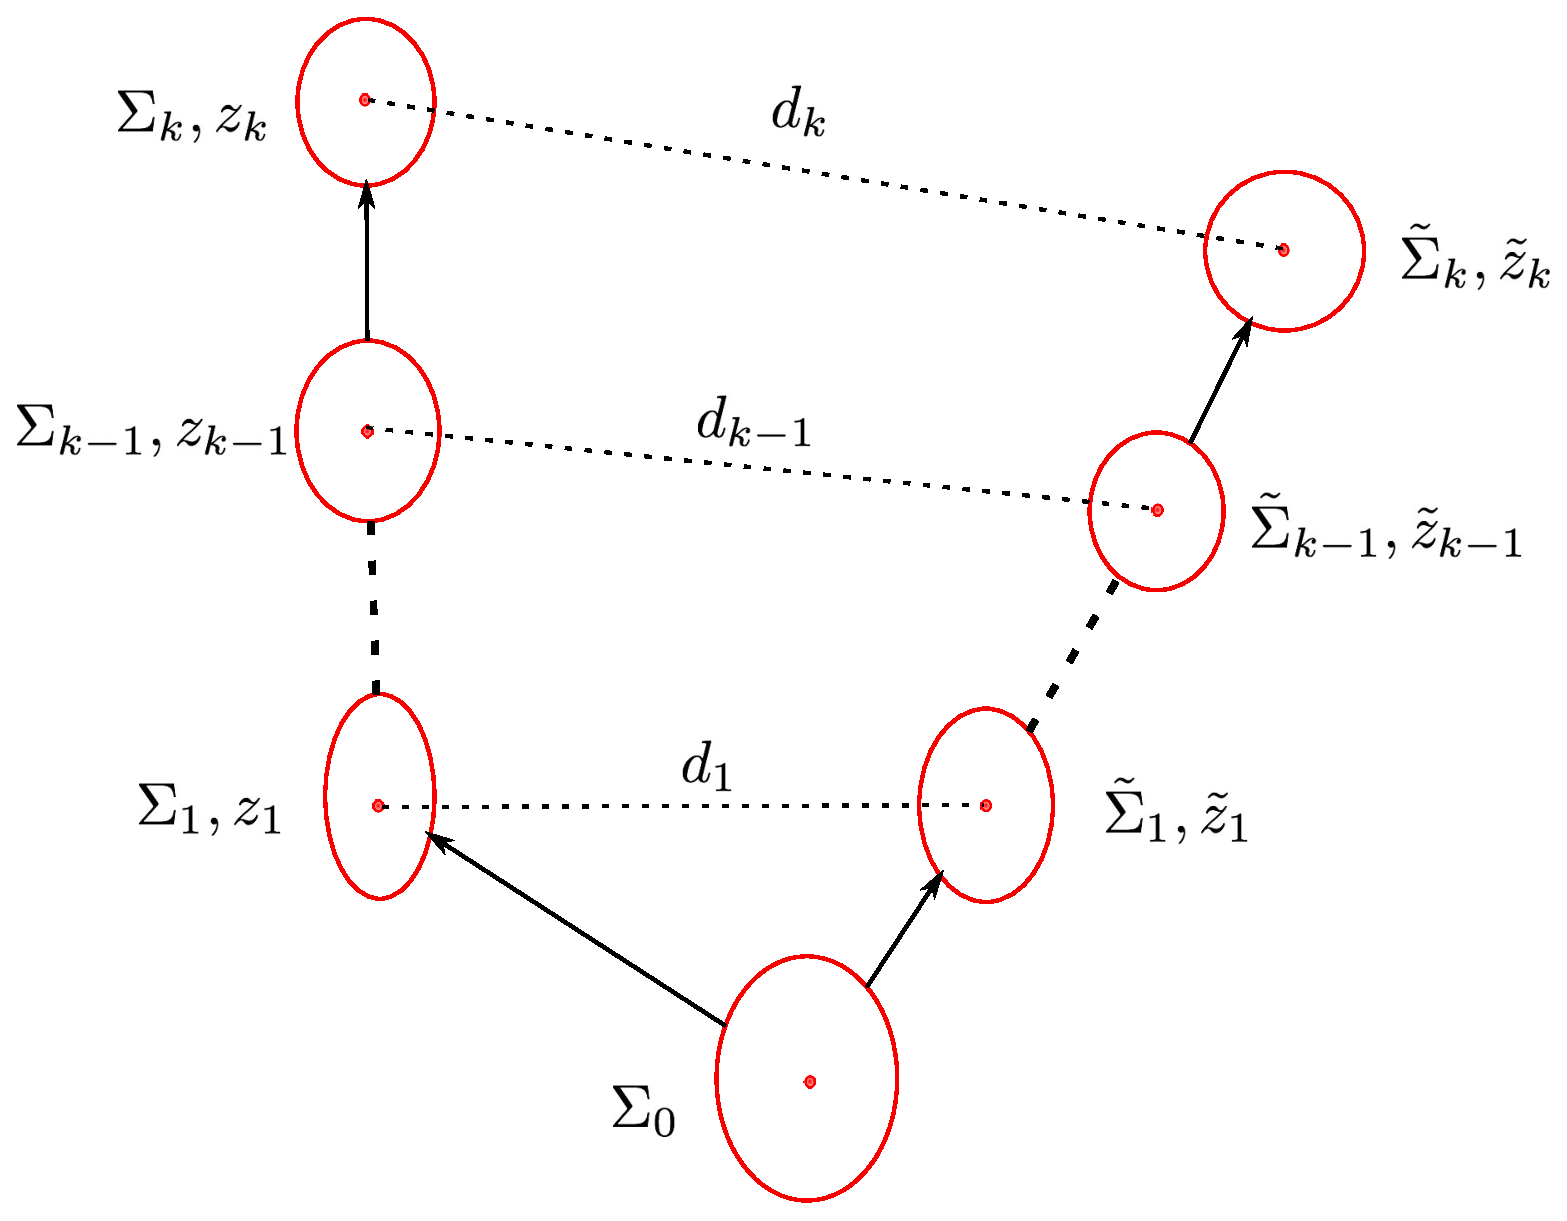
\includegraphics[width=6cm]{figs/Distance.eps}
  \caption{Distance}
  \label{Distance}
\end{figure}

We assume the robot was using a Kalman filter to estimate the target's position and the robot was not aware of the signal spoofing component $\epsilon_t$. To avoid detection, the spoofing signal cannot be too large.  Otherwise, the robot may detect abnormality and be aware the target is trying to mislead it.


We consider three problems in this paper, depending on whether the initial information available to the target or not.

\begin{problem} [Off-Line with Known Initial Condition] \label{problem1}
Given a detectable and stabilized system $\{F, H, B, Q, R \}$ from \eqref{robot}, an known initial position and covariance $(x_0, \Sigma_0)$, desired separation to avoid detection $d_1,d_2,\cdots,d_T$, discount factor $\gamma_0,\cdots,\gamma_T$. Find a sequence of spoofing signal input, $\epsilon_1, \epsilon_2,\cdots,  \epsilon_{T} $ from time $t=0$ to $t=T$ to maximize the sum of total norm of the spoofing signal from time $t=0$ to $t=T$. That is, 

\begin{equation}
  \label{eq5}
 \text{minimize}  \quad \sum^{t=T}_{t=1} \gamma_t \cdot \lVert \epsilon_t\lVert_p^p
\end{equation}
suject to,
\begin{equation} \label{problem1st}
\begin{split}
&\quad \lVert m_T - \tilde{m}_T\lVert_p \ge d_T.
     \end{split}
\end{equation}
where $\rho_{t}(\cdot)$ is the algebraic Riccati equation~\cite{kumar1986stochastic}. 
\end{problem}
%\pcomment{Change the other problems to use the $\backslash$begin\{problem\} environment}

When the initial condition of $(m_0,\Sigma_0)$ used by the Kalman filter are not know to the target, who wants to design the spoofing signal. It can be shown that the condition $\lVert m_T - \tilde{m}_T\lVert_p  \ge d_T$ can no longer be guaranteed since the measurement $z_1,\cdots,z_T$ are all with random noise. Instead of formulate the constrain condition as $\lVert m_T - \tilde{m}_T\lVert  \ge d_T$, when the initial condition $m_0 \neq \tilde{m}$ and $\tilde{\Sigma}_0 \neq \tilde{\Sigma}_0$. Instead of formulating the constrain condition  as  deterministic, problem  \ref{problem2} formulates the constrain condition with the expectation.

\begin{problem}  [Off-line with Unknown Initial Condition] \label{problem2}
Given a initial position $[\tilde{x}_0, \tilde{\Sigma}_0]$, $\lVert m_0 - \tilde{m}_0\lVert = M_0$ and  desired separation $d_T$, discount factor $\gamma_0,\cdots,\gamma_T$. Find a sequence of spoofing signal input, $\epsilon_1, \epsilon_2,\cdots,  \epsilon_{T} $ from time $t=0$ to $t=T$ to maximize the sum of total norm of the spoofing signal from time $t=0$ to $t=T$. That is, 

\begin{equation}
  \label{eq5}
 \text{minimize}   \quad \sum^{t=T}_{t=1} \gamma_t \cdot \lVert \epsilon_t\lVert_p^p 
\end{equation}
subject to,
\begin{equation} \label{problem2st} 
\begin{split}
\lVert \mathbb{E}(m_T  - \tilde{m}_T)\lVert_p  \ge d_T.\\
\end{split}
\end{equation}
\end{problem}

In problem \ref{problem2}, we assume $\lVert \mathbb{E}(m_0 - \tilde{m}_0)\lVert_p = M_0$, which indicates the expected initial bias is greater or equal than a negative value $M_0$.  As shown in theorem \ref{mk}, $m_T - \tilde{m}_T$ depends on the measurement from time $0$ to time $T$ ($z_1, z_2, \cdots,z_T$) with Gaussian noise $v_t$.


Problem \ref{problem2} describes an off-line problem with unknown initial condition, the off-line optimal problem is to find the spoofing sequence $\{ \epsilon_1, \epsilon_2,\cdots, \epsilon_T \}$ at time $t=0$. One immediate work is to extend the off-line problem to an on-line algorithm. Problem \ref{problem3} formulates an on-line problem.

\begin{problem} [On-line with Unknown Initial Condition] \label{problem3}
Given a detectable and stabilized system $\{F, H, B, Q, R \}$ from \eqref{robot}, an bias initial position $[\tilde{x}_0, \tilde{\Sigma}_0]$, current time $t$, desired separation $d_1,d_2,\cdots,d_T$, a series of measurements $\{z^{real}_1, z^{real}_2, \cdots, z^{real}_t \}$ from time $0$ to current time $t$, discount factor $\gamma_0,\cdots,\gamma_T$.  Find the spoof signal input from time $t+1$ to $T$, $\epsilon=u_{t+1}, \epsilon_1,\cdots,  \epsilon_{T}$. To maximize the sum of spoofing signal input form  time $0$ to $t$. 
\begin{equation}
  \label{eq5}
  \text{minimize}   \quad \sum^{t=T}_{t=1} \gamma_t \cdot \lVert \epsilon_t\lVert_p^p
\end{equation}
subject to,
\begin{equation}
\begin{split}
 \lVert m_T - \tilde{m}_T\lVert_p  \ge d_T.
\end{split}
\end{equation}
\end{problem}




%%%%%%%%%%%%%%%%%%%%%%%%%%%%%%%%%%%%%%%%%%%%%%%%%%%%%%%%%%%%%%%%%%%%%%%%%%%%%%%%
\section{Signal Spoofing Strategies}

\begin{theorem} \label{mk} 
Given a detectable and stabilized system $\{F, H, B, Q, R \}$ from \eqref{robot} \eqref{measurement} as the set of model parameters, the evolution of the Kalman filter gives the distributions $(m_t, \Sigma_t)$ and $(\tilde{m}_t, \tilde{\Sigma_t})$. The distance $m_t  - \tilde{m}_t$ follows,
\begin{equation} \label{mt}
\begin{split}
m_t  - \tilde{m}_t = &\prod_{i=1}^kA_i\cdot (m_0  - \tilde{m}_0) + \\
&\sum_{i=0}^{t-1} \left[ \prod_{j=i}^{t-1}A_{j+1}  (B_i + C_i) \right] +B_t + C_t
\end{split}
\end{equation}
\end{theorem}
Where,
$A_t = F - \tilde{t}_t HF,\quad B_t = (K_t-\tilde{K}_t)\left[z_t-H(Fm_{t-1}+Bu_{t-1})\right], \quad
C_t= - \tilde{K}_t \epsilon_t$.

%As shown in Proposition 1, at step $t$, the estimation error caused by the spoofing single $m_t  - \tilde{m}_t$ is a linear function of $\epsilon_1, \epsilon_2, \cdots, \epsilon_t$. Since the Kalman gain $K_t$ can be obtained from the Kalman Ricatti equation with initial condition $\Sigma_0$, thus the problem can be solved by linear programming.

Theorem \ref{mk} shows that the distance of the two estimation mean at time $t$ depends on: 1) The initial knowledge about $m_0$ and $\tilde{m}_0$. 2) The initial covariance matrix $\Sigma_0$ and $\tilde{\Sigma}_0$.

If we know the initial condition, as $m_0=\tilde{m}_0$ and $\Sigma_0 = \tilde{\Sigma}_0$,  since the covariance matrix updates through the same Ricatti equation \eqref{Riccati}, we have $\Sigma_t = \tilde{\Sigma}_t$ for all $t$. Thus, $B_t = 0$. Equation \eqref{mt} can be simplified as:
$$  m_t  - \tilde{m}_t =\sum_{i=0}^{k-1} \left(\prod_{j=i}^{k-1}A_{j+1}  C_i\right) + C_t $$
 As a result, $m_t  - \tilde{m}_t $ is independent of the measurements $z_1, z_2, \cdots, z_t$  if the estimator's initial condition is $m_0=\tilde{m}_0$ and $\Sigma_0 = \tilde{\Sigma}_0$.

Consequently, Problem \ref{problem1} can be solved off-line. Problem \ref{problem1} and Problem \ref{problem2} are generally two nonlinear programming problems for available norm p. However, when the norm is 1-norm. This section shows Problem \ref{problem1}  can both be formulated as a linear programming problem. Linear programming  can be solved in polynomial time \cite{karmarkar1984new}. On the other hand, when  2-norm is used, problem becomes a QCQP(Quadratically constrained quadratic program), which can be solved optimally. The following shows how to formulate the LP and QCQP solutions.

\begin{theorem}
Problem \ref{problem1} and Problem \ref{problem2} are linear programming problem when 
the norm is 1-norm($p=1$). And Problem \ref{problem1} and Problem \ref{problem2} are QCQP when the norm is 2-norm($p=2$).
\end{theorem}

\subsection{Linear Programming Formulation  $p=1$}
\label{p_equal_1}

 
In Problem \ref{problem1}, let $\epsilon_i=[\epsilon_i^x, \epsilon_i^y]^T$. The constraint condition $\lVert m_t-\tilde{m}_t\lVert_1 $ follows:

\begin{equation} \label{replacePro1}
\begin{split}
\lVert m_t-\tilde{m}_t\lVert_1  &=\left\lVert\sum_{i=0}^{t-1} \left(\prod_{j=i}^{t-1}A_{j+1}  C_i\right) + C_t \right\lVert_1\\
&= \left\lVert \sum_{i=0}^{t-1} \left[ \prod_{j=i}^{t-1}A_{j+1}\cdot \tilde{K}_i  \cdot \epsilon_i\right] + \tilde{K}_t \epsilon_t \right\lVert_1
\end{split}
\end{equation}
Where, $k=1,2,\cdots,T$. Since $\prod_{j=i}^{t-1}A_{t-j-1}\cdot K_i$ is constant $2 \times 2$ matrix which can be calculated from the initial covariance $\Sigma_0$ and the Riccati equation. 
And the 1-norm is simply the sum of the absolute values of the columns, (\ref{problem1st}) in Problem \ref{problem1} is a linear combination of  $\lVert \epsilon_i^x\lVert_1 $ and $\lVert \epsilon_i^y\lVert_1 $

Thus, Problem \ref{problem1} can be relaxed as a linear programming problem.


Similarly, the constraint condition (\ref{problem2st}) in Problem \ref{problem2} follows, 
\begin{equation} 
\begin{split}
& \lVert \mathbb{E}\left(m_t-\tilde{m}_t\right)\lVert_1   \\
&= \Bigg\lVert \mathbb{E} \left(\sum_{i=0}^{t-1}  \prod_{j=i}^{t-1}A_{j+1}\cdot B_i    +  B_t \right) + \\
&\quad\prod_{i=0}^{t-1}A_{t-i} \mathbb{E} (m_0  - \tilde{m}_0) +\sum_{i=0}^{t-1} \left[ \prod_{j=i}^{t-1}A_{j+1} \tilde{K}_i   \epsilon_i\right] +  \tilde{K}_t\epsilon_t \Bigg\lVert_1
\end{split}
\end{equation}

The real measurement $z_i = H(Fm_{i-1} +Bu_{i-1}+w_i)+v_i$, Where $w_i$ and $v_i$ are Gaussian noise. The expected measurement value of $\mathbb{E}(z_i)=H(Fm_{i-1}+Bu_{i-1})$ for all $i$, thus $\mathbb{E}[z_i-H(Fm_{i-1}+Bu_{i-1})]=0$. Since $\lVert \mathbb{E}(m_0-\tilde{m}_0)\lVert_1  = M_0$ and $\mathbb{E}[B_i] = 0$, then
\begin{equation}
\begin{split}
& \lVert \mathbb{E}\left(m_t-\tilde{m}_t\lVert_1  \right)\\
&=  \Bigg\lVert M_0\prod_{i=0}^{t-1}A_{t-i} +\sum_{i=0}^{t-1} \left[\prod_{j=i}^{t-1}A_{j+1} \tilde{K}_i \epsilon_i\right] +  \tilde{K}_t\epsilon_t \Bigg\lVert_1
\end{split}
\end{equation}

As a result, the  inequality  constraint condition (\ref{problem2st}) can be formulated as a linear combination of $\lVert \epsilon_i\lVert_1 $:   
\begin{equation} \label{replacePro2}
\Bigg\lVert M_0\prod_{i=0}^{t-1}A_{t-i} +\sum_{i=0}^{t-1} \left[\prod_{j=i}^{t-1}A_{j+1} \tilde{K}_i \epsilon_i\right] +  \tilde{K}_t\epsilon_t \Bigg\lVert_1 \ge d_t
\end{equation}

\subsection{Quadratically Constrained Quadratic Program Formulation $p=2$}
If we consider the distance as Euclidean distance, the norm would be 2-norm. It can be shown that the problem is a Quadratically Constrained Quadratic Program(QCQP)\cite{boyd2004convex}, a problem closely related to quadratic programming. The standard from of QCQP is:
\begin{equation}
\begin{split}
\text{minimize} \quad &\frac{1}{2} X^TP_0X+q_0^TX+r_0\\
\text{subject to:}\quad &\frac{1}{2} X^TP_iX+q_i^TX+r_i,\quad i=1,\dots,T\\
&Lx=g
\end{split}
\end{equation}
Where $X\in \mathbb{R}^n$ is the optimization variable, $A_i\in \mathbb{R}^{n_i \times n}$, $F \in \mathbb{R}^{p\times n}$.

Thus, in problem \ref{problem1}, let $X=[\epsilon^x_{1},\epsilon^y_{1},\cdots,\epsilon^x_{T},\epsilon^y_{T}]\in \mathbb{R}^{2T}$. The objective function $\sum_{i=1}^T \lVert \epsilon_i \lVert_2^2$ follows a quadratic function and $\beta,L,g =0$. Matrix $P_T$ and $q_T$  could be obtained from a transformation from the following matrix: $$\left[\prod_{j=0}^{T-1}A_{j+1} \tilde{K}_0,\cdots, \prod_{j=T-1}^{T-1}A_{j+1} \tilde{K}_{T-1}, {K}_T \right]$$
since $\lVert Ax-b \lVert_2=x^TA^TAx-2b^TAx+b^Tb$.


As shown above, when $p=2$. Problem \ref{problem1} is equivalent to QCQP.

In problem \ref{problem2}. The only difference is $M_0\prod_{i=0}^{t-1}A_{t-i}$ is added. Similarly, it is also a QCQP.

%%%%%%%%%%%%%%%%%%%%%%%%%%%%%%%%%%%%%%%%%%%%%%%%%%%%%%%%%%%%%%%%%%%%%%%%%%
\section{Simulations}
Consider a system:
$$ x_{t+1}=\left[\begin{matrix}
   0.9 & 0.2 \\
   0.3 & 0.85 \\
  \end{matrix} \right] x_{t}+u_t+\omega_t, \omega_t \sim (0,0.1)$$

%%%%%%%%%%%%%%%%%%%%%%%%%%%%%%%%%%%%%%%%%%%%%%%%%%%%%%%%%%%%%%%%%%%%%%%%%%
\section{Conclusion} \label{sec:conc}

%%%%%%%%%%%%%%%%%%%%%%%%%%%%%%%%%%%%%%%%%%%%%%%%%%%%%%%%%%%%%%%%%%%%%%%%%%
\appendix

\subsection{Kalman filter and Ricatti equation}
Suppose the true measurement is $z(t)$, the Kalman filter estimation is:
\begin{align}
\label{filter}
&\hat{x}_{t|t-1} = Fx_{t-1|t-1} + Bu_t\\
&\hat{x}_{t|t}=F\hat{x}_{t|t-1}+K_t(z_t-H\hat{x}_{t|t-1}\\ 
&\hat{\Sigma}_{t|t}=(I - K_t H_t) ( F \hat{\Sigma}_{t|t-1} F' + R_t )
\end{align}
Where $K_t$ is the Kalman gain and is given by:
\begin{equation}
\label{kalman_gain}
K_t = (F \hat{\Sigma}_{t|t-1} F' + R_t)H'(H \Sigma_{t|t-1} H' + Q_t )^{-1}
\end{equation}

From the Kalman gain update equation (\ref{kalman_gain}), the evolution covariance matrix at step $t$, and $\Sigma_t$ only depends on the state model parameters and the initial condition of the covariance matrix $\Sigma_0$. And the Kalman gain at step $t$, $K_t$ depends on the covariance matrix $\Sigma_t$. They do not depend on the control input series $\{u_t\}_{t=1,\cdots,k}$, measurement $\{z_t\}_{t=1,\cdots,k}$. Thus, the covariance matrix and the Kalman gain can be predict from the discrete Riccati difference equation \cite{kumar1986stochastic}.
\begin{equation} \label{Riccati}
\begin{split}
\hat{\Sigma}_{t+1}=&F\hat{\Sigma}_tF^T-F\hat{\Sigma}_tH_{t}^T(H\hat{\Sigma}_tH^T+Q_t)^{-1}H\hat{\Sigma}_tF^T\notag\\
 &+R_t 
 \end{split}
\end{equation}

\subsection{Proof of theorem \ref{mk}}
Statement of theorem \ref{mk}: 


\proof From the update of Kalman filter, we have
\begin{equation}
\begin{split}
\label{Proposition1}
 m_t& = m_{t|t-1} + K_t(z_t-Hm_{t|t-1})\\
&=(I-K_tH)m_{t|t-1} +K_t z_t\\
&=(I- K_tH) (Fm_{t-1}
+Bu_{u-1}) +K_t z_t
\\
\end{split}
\end{equation}
And
$$\tilde{m}_t = (I- K_tH) (Fm_{t-1} +Bu_{u-1}) +K_t (z_t + \epsilon_t)$$
Induction on this yields:
\begin{equation}
\begin{split}
\label{Proposition2}
m_t & - \tilde{m}_t \\
=& (I- K_tH) (Fm_{t-1} +Bu_{u-1}) +K_t z_t \\
&- [(I- \tilde{K}_tH) (F\tilde{m}_{t-1} +Bu_{u-1}) +\tilde{K}_t (z_t+\epsilon_t)]\\
=& (F - K_t H F)m_{t-1} - (F- \tilde{K}_t H F)\tilde{m}_{t-1}\\
&-(K_t - \tilde{K}_t)HBu_{t-1} + [K_t z_t - \tilde{K}_t(z_t+ \epsilon_t)]\\
=& (F - \tilde{K}_tHF)m_{t-1} - (F- \tilde{K}_tHF)m_{t-1}\\
&- (K_t - \tilde{K}_t) H Bu_{t-1} +(K_t - \tilde{K}_t)z_t - \tilde{K}_t \epsilon_t\\
&-(K_t - \tilde{K}_t) HFm_{t-1}\\
=&(F - \tilde{K}_t HF)(m_{t-1} - \tilde{m}_{t-1})\\
&+(K_t - \tilde{K}_t)[z_t - H (Fm_{t-1} + Bu_{t-1})] -\tilde{K}_t \epsilon_t
\end{split}
\end{equation}

Let,
$$A_t = F - \tilde{K}_t HF$$
$$B_t = (K_t-\tilde{K}_t)[z_t-H(Fm_{t-1}+Bu_{t-1})]$$
$$C_t = - \tilde{K}_t \epsilon_t$$
Then,
\begin{equation}
\begin{split}
\label{Proposition2}
m_t  -& \tilde{m}_t \\
=& A_t (m_{t-1} - \tilde{m}_{t-1}) + B_t + C_t\\
=& A_t[A_{t-1}(m_{t-1} - \tilde{m}_{t-1}) + B_{t-1} + C_{t-1}]\\
\qquad \vdots \\
=&\prod_{i=t}^tA_i\cdot (m_0  - \tilde{m}_0)+ \\
&(B_t + C_t) + A_t (B_{t-1}+C_{t-1}) \\
&+  A_t A_{t-1}(B_{t-2}+C_{t-2}) \cdots \\
&+ A_t \cdots A_3 A_2 A_1(B_0 + C_0)  \\
= &\prod_{i=t}^tA_i\cdot (m_0  - \tilde{m}_0) + \\
&\sum_{i=0}^{t-1} \left[ \prod_{j=i}^{t-1}A_{j+1} (B_i + C_i) \right] +B_t + C_t
\end{split}
\end{equation}



\bibliographystyle{plain}
\bibliography{main}


\end{document}
